\univlogo

{\Huge March 21}\vspace{5mm}

\section*{Configure working environment}

\subsection*{Download plugins for Latex in VSCode}

Use linux commands to install Latex:

\begin{lstlisting}[language=bash]
    sudo pacman -s texlive-most
\end{lstlisting}

Install LaTeX Workshop plugin from the Visual Studio Code Marketplace.

\begin{figure}[h]
\centering

\includegraphics[width=1\textwidth]{./2023Mar/LaTeX-Workshop.png}
\caption{A Latex plugin in VSCode market}
\label{latexworkshop}
\end{figure}

\subsection*{Create a LaTeX project}

Select a place in your PC and create a directory.

Change your workspace into the directory and create a main.tex file in which you will edit your LaTeX code.

\subsection*{LaTeX+Git}

\emph{'If you are only editing it locally, it is just as simple as creating any other repository. But this starts shining when you want to work with others, or you want people to be able to check your work without you heaving to send it to them every time. On top of that, uploading your content to a remote GIT repository can protect you in case of a catastrophic failure in your personal machine.'}

\href{https://medium.com/@rcpassos/writing-latex-documents-in-visual-studio-code-with-latex-workshop-d9af6a6b2815}{Writing LaTeX Documents In Visual Studio Code With LaTeX Workshop} 

Ahead of all, we should change local git branch name to main:

\begin{lstlisting}[language=bash]
    git config --global init.defaultBranch main
\end{lstlisting}

Then we can do the following to push out LaTeX project to the git repository:

\begin{lstlisting}[language=bash]
    git init
    git add .
    git commit -m "My first try to sync overleaf with Github"
    git remote add origin https://github.com/username/repo
    git push -u origin main
\end{lstlisting}

\emph{'It is recommended to use a \href{https://github.com/github/gitignore/blob/main/TeX.gitignore}{.gitignore file} to keep your repository free of temporary files, and any side products created during compilation.'}

\subsection*{Synchronize overleaf with Github}

When creating a new project, there is a option to import it from Github:

\begin{figure}[h]
\centering
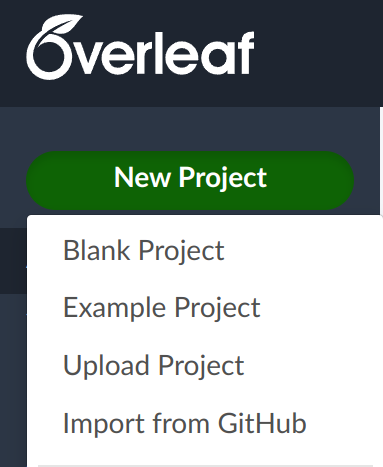
\includegraphics[width=0.3\textwidth]{./2023Mar/Import-From-Github.png}
\caption{Import overleaf project from Github}
\label{importfromgithub}
\end{figure}

However, this feature works only for premium users. It costs 9\$ per month for students to get access to this feature.

\subsection*{Enjoy the fast editor and preview now}

With all these done, you can just edit your LaTeX project locally and compile much more faster than what overleaf does. Just update your projects by using git and sync your project on overleaf by clicking a blue button.

